\documentclass[10pt,twocolumn,letterpaper]{article}

\usepackage{cvpr}
\usepackage{times}
\usepackage{epsfig}
\usepackage{graphicx}
\usepackage{amsmath}
\usepackage{amssymb}
\usepackage{subcaption}

% Include other packages here, before hyperref.

% If you comment hyperref and then uncomment it, you should delete
% egpaper.aux before re-running latex.  (Or just hit 'q' on the first latex
% run, let it finish, and you should be clear).
\usepackage[breaklinks=true,bookmarks=false]{hyperref}

\cvprfinalcopy

% \def\cvprPaperID{****} % *** Enter the CVPR Paper ID here
\def\httilde{\mbox{\tt\raisebox{-.5ex}{\symbol{126}}}}

% Pages are numbered in submission mode, and unnumbered in camera-ready
%\ifcvprfinal\pagestyle{empty}\fi
\setcounter{page}{1}
\begin{document}

%%%%%%%%% TITLE
\title{
    Better Image Super-Resolution Using Semantic Segmentations \\
    \large CS 381V Visual Recognition Final Project}

\author{Keivaun Waugh\\
University of Texas at Austin\\
{\tt\small keivaunwaugh@gmail.com}
\and
Paul Choi\\
University of Texas at Austin\\
{\tt\small choipaul96@gmail.com}
}

\maketitle

%%%%%%%%% ABSTRACT
\begin{abstract}
    In this paper, we address the problem of image super-resolution (SR) using
    a ResNet-based convolutional neural network (CNN) as well as a generative
    adversarial network (GAN). We build upon these prior approaches to SR by
    utilizing semantic segmentation data as an additional signal for the neural
    network. We first experiment with human-annotated pixel-wise segmentations
    as a proof-of-concept, and additionally experiment with machine-generated
    pixel-wise segmentations to demonstrate a fully-automated approach that
    does not require human annotations. Our results show that using
    segmentation data increases both quantitative and qualitative performance
    of neural networks for the super-resolution task.
\end{abstract}

%%%%%%%%% BODY TEXT
\section{Introduction}
Image super-resolution is a compelling area of computer vision. The ability to
convert low-resolution photos and video to higher resolution counterparts
becomes more valuable as today's hardware continues to improve. Cameras and
displays constantly improve their resolution, and as they overtake earlier
technology, media created using older devices look more dated. This makes it
desirable to convert older media to the same resolution standards as current
photos and videos.

Unlike image downsampling, its counterpart task, SR is an inherently
underspecified problem as the dimensionality of the output exceeds that of the
input. The goal of a good SR solution is to define a transformation that
``hallucinates'' information from the low-resolution (LR) image to fill in the
gaps for the high-resolution (HR) image. Naive methods of upsampling using
nearest neighbor or bicubic interpolation introduce many artifacts and produce
visually displeasing images.

To evaluate a SR approach, a downsampled instance of an image is used as input,
and the original image is used as ground truth for evaluating the output. Naive
methods of SR are unconvincing and indicate immediately to the viewer that the
image has been upscaled. Stronger SR approaches produce images which require
closer inspection to recognize as upscaled, and perfect solutions are
indistinguishable from ground truth.

\begin{figure}[ht]
    \begin{tabular}{cc}
        Ours & Original \\
        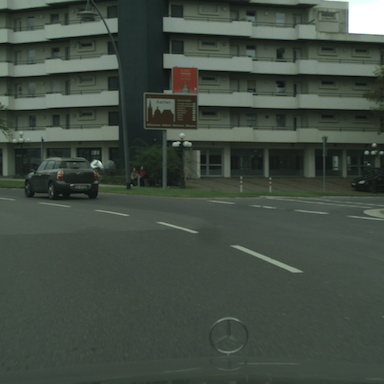
\includegraphics[trim=0 0 0 0, clip,
            width=1.5in]{images/example_hr_image.png} &
        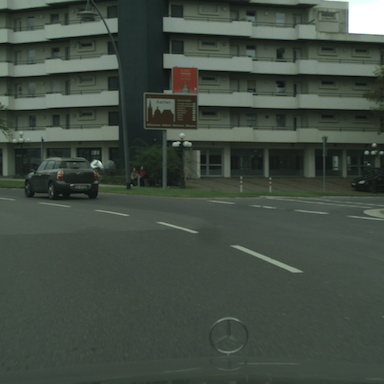
\includegraphics[trim=0 0 0 0, clip,
            width=1.5in]{images/example_hr_image.png} \\
    \end{tabular}
    \caption{Our super-resolved image (left) compares favorably to the original
    image (right).}
    \label{fig:exampleIntroFirst}
\end{figure}

Deep neural networks (DNNs) have greatly increased in popularity for the
instance and category recognition tasks, sparked by work from Krizhevsky et al.
\cite{AlexNet}. Recently, DNNs have also achieved considerable success in the
SR task. We use previous DNN approaches as a foundation for our work. In this
paper, we combine semantic segmentation features with state-of-the-art deep SR
techniques in order to achieve sharper and more convincing SR results.

\begin{figure*}[ht!]
    \begin{center}
        \begin{tabular}{cccc}
            Bicubic & SRResnet & With Machine Segmentation &
            With Human Segmentation \\
            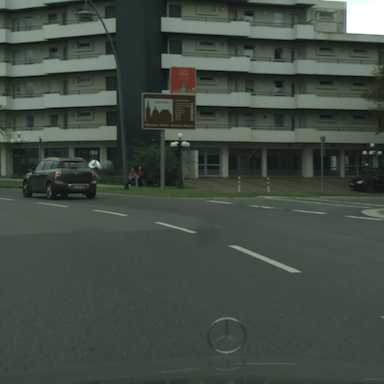
\includegraphics[trim=0 0 0 0, clip,
                width=1.5in]{images/segmentation_original.png} &
            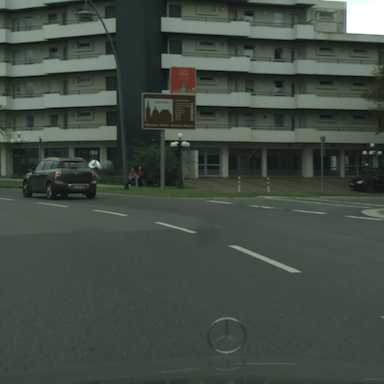
\includegraphics[trim=0 0 0 0, clip,
                width=1.5in]{images/segmentation_original.png} &
            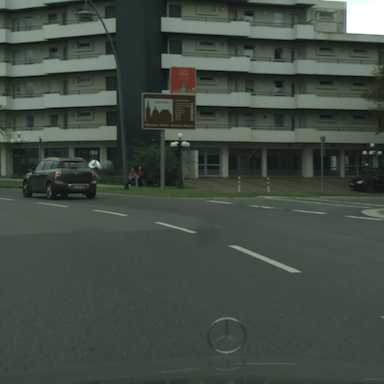
\includegraphics[trim=0 0 0 0, clip,
                width=1.5in]{images/segmentation_original.png} &
            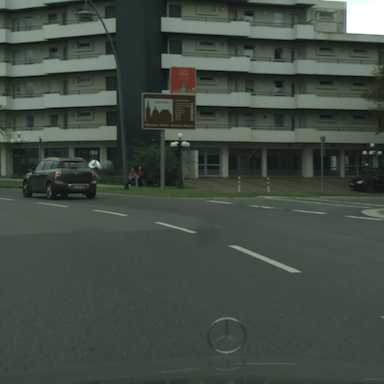
\includegraphics[trim=0 0 0 0, clip,
                width=1.5in]{images/segmentation_original.png} \\
            Nearest Neighbor & SRGAN & With Machine Segmentation &
            With Human Segmentation \\
            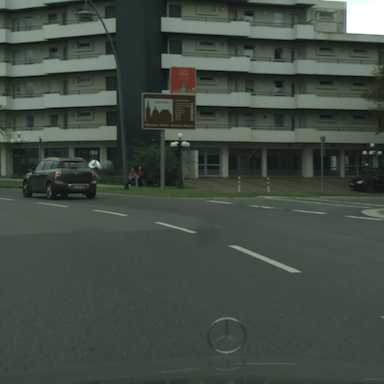
\includegraphics[trim=0 0 0 0, clip,
                width=1.5in]{images/segmentation_original.png} &
            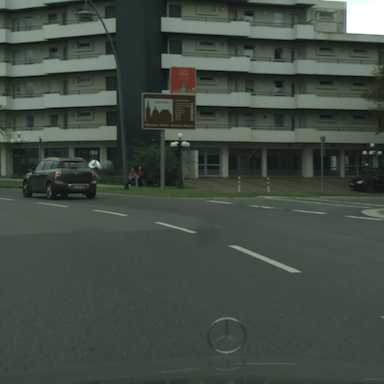
\includegraphics[trim=0 0 0 0, clip,
                width=1.5in]{images/segmentation_original.png} &
            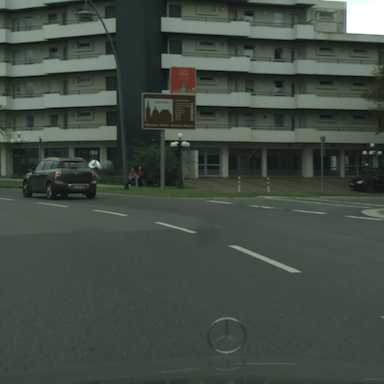
\includegraphics[trim=0 0 0 0, clip,
                width=1.5in]{images/segmentation_original.png} &
            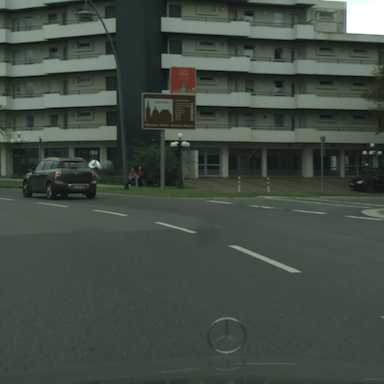
\includegraphics[trim=0 0 0 0, clip,
                width=1.5in]{images/segmentation_original.png}
        \end{tabular}
    \end{center}
    \caption{Comparison of bicubic and nearest neighbor interpolation, prior
    DNN-based approaches, and our approach using human segmentations.}
    \label{fig:methodComparison}
\end{figure*}

%------------------------------------------------------------------------------

\subsection{Related Work}
Basic approaches to SR existed before the advent of deep neural networks.  The
most naive is nearest neighbor interpolation, which assigns pixels in the
output image by selecting the spatially nearest corresponding pixel in the
input image. A more common, superior method which is the standard in many image
editors is bicubic interpolation, which computes output pixel values as the
weighted average of a corresponding neighborhood of input pixels. However,
neither of these methods attempt to use any kind of local or global structure
in the image or domain knowledge to perform a better reconstruction.

Other, more advanced, non-deep approaches exist for SR. Chung et al.
\cite{FractalSR} investigate the use of fractal patterns for the task of
super-resolution. Approaches for SR optimized for video exist, such as those
mentioned in Borman and Stevenson's review \cite{VideoSR}. These algorithms use
the content of neighboring frames to to intelligently compute values for the
output pixels. In this work, we only consider the problem of single image SR.

Dong et al. \cite{SRCNN} were the first to propose a convolutional neural
network (CNN) for the purpose of SR.  They used a basic deep architecture and
trained their model end-to-end using a per-pixel loss between the output and
ground truth images. Johnson et al.  \cite{PerceptualLosses} proposed the use
of a perceptual loss function based on high-level features of neural networks
to make the images more appealing to eye. They achieve worse quantitative
results in metrics such as peak signal-to-noise-ratio (PSNR) and structural
similarity (SSIM), but better qualitative results. This helped to motivate
future work to use perceptual metrics such as mean opinion score (MOS). Other
work involving CNNs for SR include \cite{RealtimeCNN} and
\cite{DeeplyRecursive}.

Another recent approach uses a generative adversarial network (GAN) \cite{GAN}.
As previously mentioned, the CNN approaches typically attempt to minimize the
per-pixel loss between the upsampled output image and the original unmodified
image. The error metric frequently used is peak signal-to-noise ratio (PSNR).
However, when this is applied directly on the pixel space, it often
encourages the network to make soft changes in the upsampled image rather than
generate the high-frequency changes typically found in images. GAN-based
approaches like the work of Ledig et al. \cite{SRGAN} attempt to overcome this
by using an adversarial network. Though they have lower PSNR scores, the images
often look more realistic, which suggests that a different metric should be
optimized to get higher-quality results.

The semantic segmentation task involves predicting, at each pixel of an input
image, the semantic class of the enclosing object or region from a predefined
set of classes. Long and Shelhamer et al. \cite{FullyConvolutionalSS} proposed
a robust CNN solution for the task.

In \cite{ImageSynthesis}, Chen and Koltun experiment with using semantic
segmentation from the Cityscapes dataset \cite{Cityscapes} to perform
photorealistic image synthesis. The authors produce images of photographic
quality using only the semantic segmentations as input to their CNN. To our
knowledge, semantic segmentation data has not been utilized for the SR task.

\subsection{Motivation}
Chen and Koltun achieve extremely realistic results for image synthesis using
solely semantic segmentation data. Their approach has extremely high capacity
for learning how to synthesize objects and regions based on their semantic
class and what it sees during training. We believe that this ability can be
utilized in super-resolution networks to produce more realistic upsamplings. In
discussions with our peers, some argued that the network should learn object
boundaries and semantic classes and incorporate this data on its own. However,
we know that DNNs often need human intervention in order to learn in a certain
way. One example of this is residual networks \cite{ResNet}. The intuition
behind the benefit of ResNets and the skip connections used is that they assist
the network in learning identity mappings when they are optimal. Theoretically
a layer can learn identity mappings, but it is much easier to do so when there
is a skip connection. Similarly, we believe that explicitly providing semantic
segmentations will guide the network in learning semantic class-specific
knowledge and utilizing the class boundaries.

\subsection{Contribution}
In this paper, we believe we are the first to explore how the addition of
pixel-wise semantic segmentation masks affect a network's ability to
super-resolve images. We experiment with a high upscaling factor ($4 \times$).
We hypothesize that segmentations will assist the network in making intelligent
decisions at object boundaries, as well as in learning how to realistically
upsample different semantic classes. We evaluate the impact of these
segmentations on the ResNet-based and GAN-based SR architectures proposed by
Ledig et al. \cite{SRGAN}.

We describe our network architecture and segmentation pipeline in section
\ref{sec:method}. A quantitative and qualitative evaluation of results is
included in section \ref{sec:results}. Section \ref{sec:conclusion} contains
concluding remarks and directions for future work based on our segmentation
approach.

%------------------------------------------------------------------------------

\section{Method}
\label{sec:method}

Our approach uses a standard convolutional neural network based on the ResNet
architecture \cite{ResNet} as well as generative adversarial networks
\cite{GAN}. These architectures were originally proposed by Ledig et al. in
\cite{SRGAN}. We modify the input layer of the networks to include, in addition
to the RGB channels of the image, the \textit{semantic layout} of the image
following Chen and Koltun \cite{ImageSynthesis}. The semantic layout is defined
as $L \in \{0, 1\}^{m \times n \times c}$ where $m \times n$ is the image
resolution and $c$ is the number of semantic classes. Each pixel in the image
corresponds to a one-hot vector in $L$ indicating its semantic class: $L(i, j)
\in \{0, 1\}^c$ s.t. $\sum_p L(i, j, p) = 1$.

This approach assumes that the network is trained and evaluated on the same set
of semantic classes. In other words, during training and testing each channel
of the semantic layout provided to the network must be of the same classes in
the same order. Using different semantics in the layout could negatively affect
training. While this adds some restrictions to our SR approach, it also allows
for additional flexibility in image domain. If the network will be used for a
very specific domain (e.g. streetview images only), an appropriately narrow set
of semantic classes can be used to sharpen the focus of the network and allow
for faster training. For more general domains, a wider and more inclusive set
of classes can be used.

\begin{figure*}[ht!]
\begin{center}
    \begin{tabular}{c}
	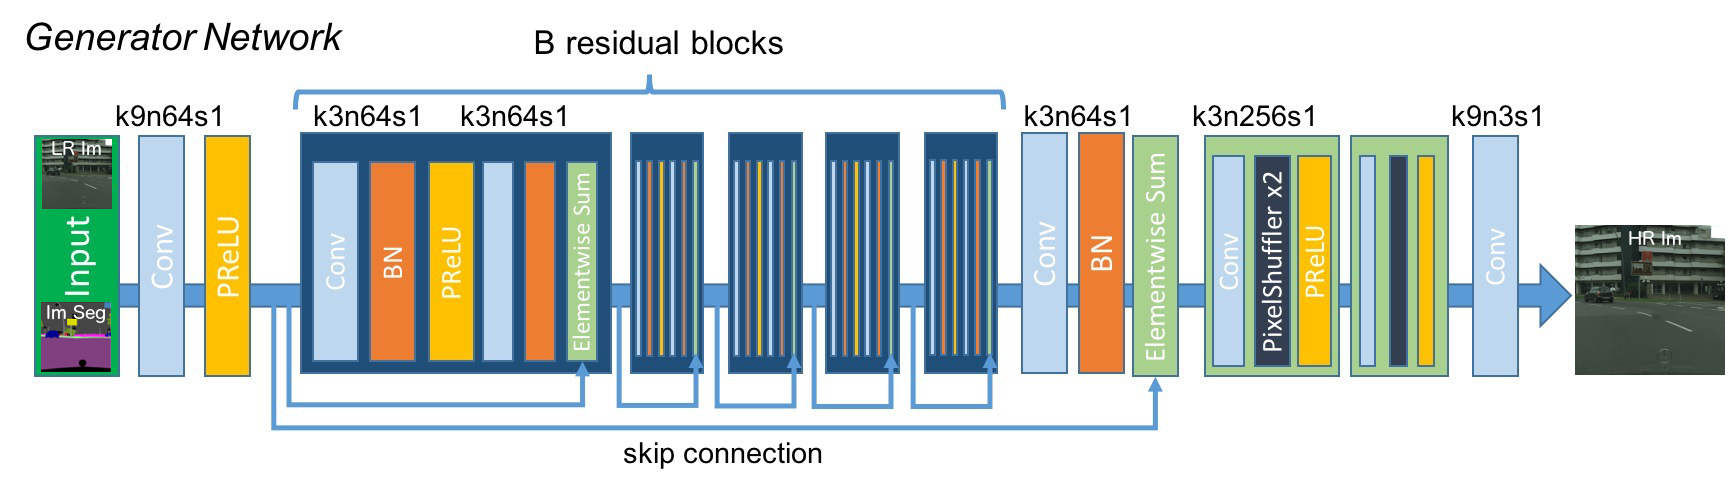
\includegraphics[width=6.5in]{images/generator_architecture.png} \\
	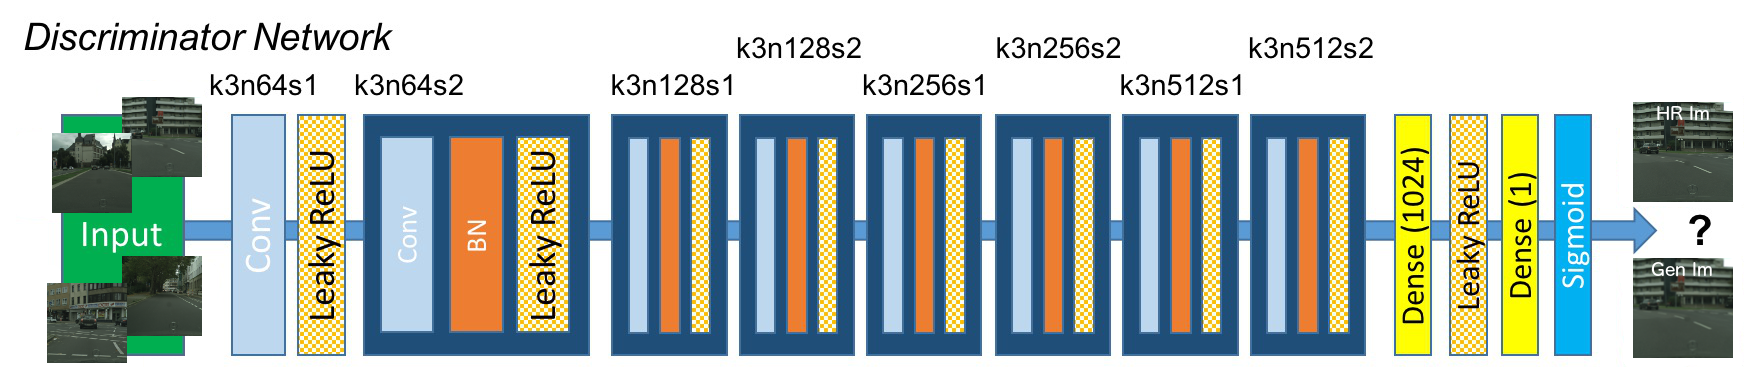
\includegraphics[width=6.5in]{images/discriminator_architecture.png}
    \end{tabular}
\end{center}
    \caption{Architecture of Generator and Discriminator Network with kernel
    size (k), feature map count (n), and stride (s) at each layer in the
    network. Diagrams courtesy of \cite{SRGAN}.}
    \label{fig:architecture}
\end{figure*}

Figure \ref{fig:architecture} illustrates the architectures for the generator and
the discriminator. When training the GAN-based network, the generator is
pretrained for $n$ epochs, after which the generator and discriminator are
jointly trained for $m$ epochs. We sum the mean squared error (MSE) loss,
perceptual loss, and adversarial loss for our loss function. For the
ResNet-based network, only the generator is trained, using the sum of the MSE
loss and perceptual loss.

To perform a forward and backward pass, we take an image and downsample it by a
scale factor of 4. We concatenate the downsampled image with the semantic
layout as input to the network. For the backward pass, the losses are
calculated using the original image as ground truth.

\subsection{Human Segmentations}
To evaluate the plausibility of our approach, we first experimented with using
human-annotated segmentations. These pixel-wise segmentations are close to
perfect; if there are any gains to be made with using segmentations, they would
be most evident with human annotations. Conversely, no improvement using human
annotations suggests that this approach should be reevaluated before further
exploration. We primarily use the Cityscapes \cite{Cityscapes} dataset in our
experiments as it includes pixel-wise human-annotated segmentations. In
Cityscapes, the number of semantic classes $c = 34$, meaning the input layer of
our network has 37 channels in our experiments. An example of a human-annotated
segmentation can be seen in \ref{fig:segmentations}.

\subsection{Machine Segmentations}
Our SR approach would be infeasible if it required human-annotation for each
image it super-resolved. To be robust, the network should be fully-automatic
--- that is, able to operate on segmentations which are machine-generated
rather than human-annotated. The segmentation network used could be optimized
for a particular domain, or be trained as a more general out-of-the-box
solution. We focus on the latter type of segmentation network in this work for
two reasons. First, we wish to show that our method is generalizable, and that
its performance is not a result of tailoring it to one particular domain.
Second, similar to the expected gap in performance gains between using
machine-generated segmentations and human-annotated segmentations, we expect
that our method will only perform better if it is trained and evaluated on a
specific domain.

We use a Fully Convolutional Network \cite{FullyConvolutionalSS} trained on the
ADE20K dataset \cite{ADE20K} in our experiments. ADE20K has a diverse
collection of scene and object categories, making our segmentation network an
out-of-the-box solution ready to be used on many different scene types.
ADE20K has 150 semantic classes. To provide a fair comparison between human
segmentations and machine segmentations, we only include the 34 most common
classes in our semantic layout to match the number of classes in Cityscapes. An
example segmentation of a Cityscapes image produced by this network can be seen
in \ref{fig:segmentations}.

We use FCNs rather than more recent state-of-the-art segmentation networks
because it is the most well-known and has easily accessible implementations. As
the performance of segmentation networks approaches human accuracy, we expect
that the performance of our fully-automated SR method to approach that of our
human-annotation method.

\begin{figure*}[t!]
    \begin{center}
        \begin{tabular}{ccc}
            Original & Human Segmentation & Machine Segmentation \\
            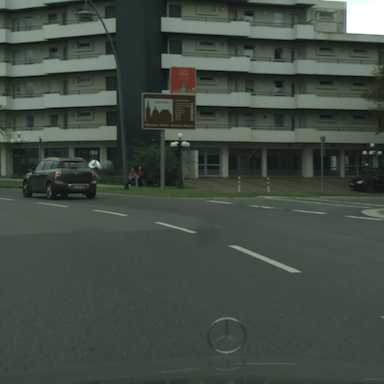
\includegraphics[trim=0 0 0 0, clip,
                width=2.0in]{images/segmentation_original.png} &
            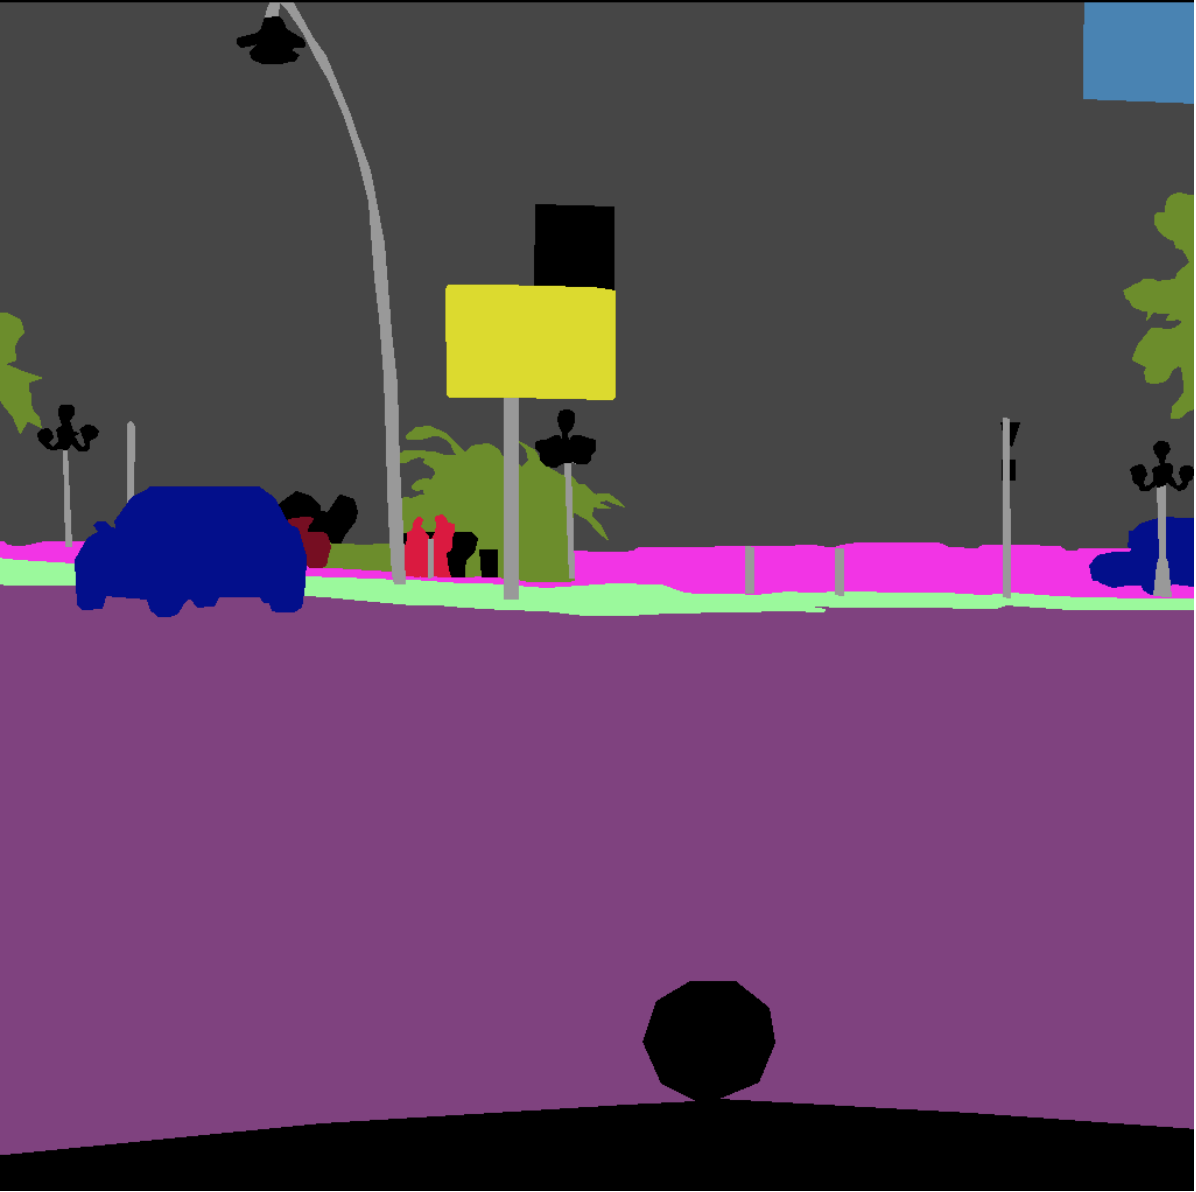
\includegraphics[trim=0 0 0 0, clip,
                width=2.0in]{images/segmentation_human.png} &
            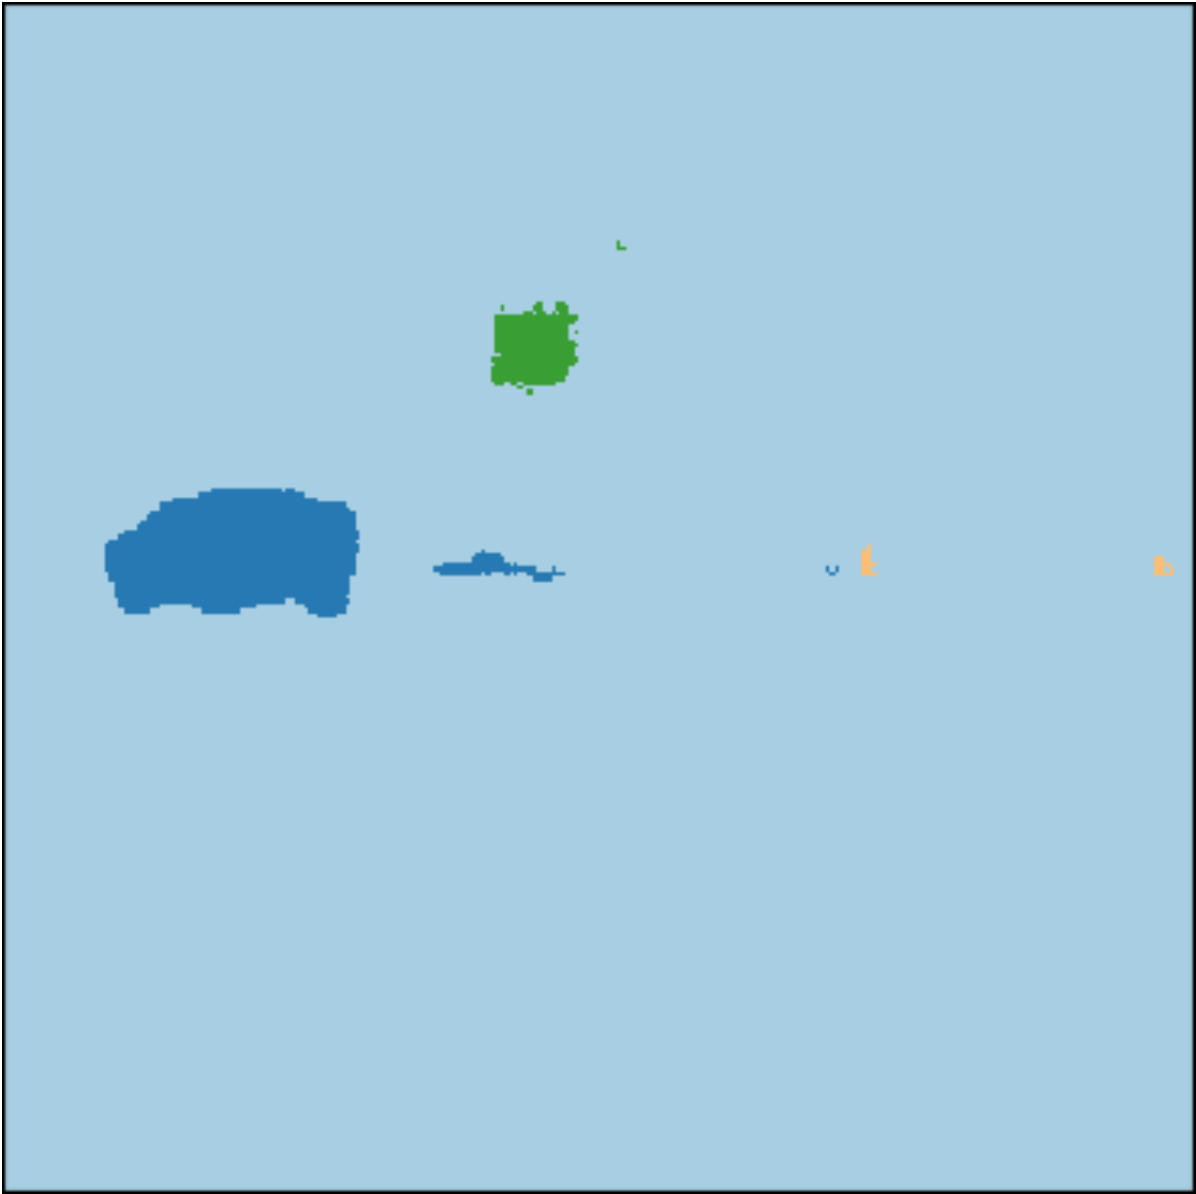
\includegraphics[trim=0 0 0 0, clip,
                width=2.0in]{images/segmentation_machine.png} \\
        \end{tabular}
    \end{center}
    \caption{Comparison of segmentations between human generated
    and auto generated. Left: The original image. Middle: A human
    annotated pixel-wise semantic segmentation. Right: A machine
    generated segmentation.}
    \label{fig:segmentations}
\end{figure*}

%------------------------------------------------------------------------------

\section{Experiments}
\label{sec:results}

\subsection{Quantitative metrics}
As is standard in other works in this domain \cite{SRCNN, SRGAN,
PerceptualLosses, DeeplyRecursive}, we use peak signal-to-noise ratio (PSNR)
and structural similarity (SSIM) as our quantitative measurements. All of our
experiments are performed with a $4 \times$ upscaling factor. We use Cityscapes
for the majority of our experiments, but we also experiment with ADE20K to
demonstrate how a segmentation network optimized for a particular dataset might
perform. Our baselines are SRResNet and SRGAN (the ResNet- and GAN-based
approaches of \cite{SRGAN}). Tables \ref{fig:quantResultsCityscapes} and
\ref{fig:quantResultsADE} show the results of thexe experiments.

\begin{figure*}[ht!]
    \begin{centering}
        \small
        \begin{tabular}{c ccccccc}
            \textbf{Cityscapes} & Bicubic & SRGAN & SRGAN (machine) & SRGAN
            (human) & SRResNet & SRResNet (machine) & SRResNet (human) \\
            \hline
            PSNR & 25.405 & 26.48 & 26.72 & 26.95 & 27.44 & 26.99 &
            \textbf{27.59} \\
            SSIM & 0.805 & 0.80 & 0.809 & 0.811 & 0.840 & 0.839 &
            \textbf{0.850}
        \end{tabular}
    \end{centering}
    \caption{Comparison of baselines and our method using Cityscapes. Highest
    measures in bold. Machine indicates machine segmentations, human indicates
    human segmentations.}
    \label{fig:quantResultsCityscapes}
\end{figure*}

\begin{figure*}[ht!]
    \begin{center}
        \small
        \begin{tabular}{c cc}
            \textbf{ADE20K} & Bicubic & SRGAN (human) \\
            \hline
            PSNR & 24.85 & \textbf{26.19} \\
            SSIM & 0.75 & \textbf{0.78}
        \end{tabular}
    \end{center}
    \caption{Comparison of baselines and our method using ADE20K.}
    \label{fig:quantResultsADE}
\end{figure*}

Ledig et al. \cite{SRGAN} found that their best approach quantitatively to be
SRResNet, the purely ResNet-based approach which does not use an adversarial
loss. We find that our best approach is SRResNet modified to use human
segmentations. Both human and machine segmentations also improve the
performance of SRGAN, while machine segmentations did not improve SRResNet.

TODO: ADE20K results discussion.

\subsection{Mean opinion score (MOS) testing}
We performed a MOS test to evaluate the quality of our approach using human
perception rather than quantitative metrics, as \cite{SRGAN} has found that
better quantitative measurements do not necessarily translate to increases in
perceptual quality. Following \cite{SRGAN}, we asked 10 raters to rate the
quality of various image on a scale of 1 to 5. We calibrated the raters by
showing them images upsampled using nearest neighbor interpolation (score of 1)
as well as the ground truth images (score of 5). Each rater rated versions of
images upsampled using nearest neighbor and bicubic interpolation, SRResNet,
SRGAN, and different variations of our approach using human and machine
segmentations, as well as the ground truth images. Raters were unaware of the
different methods being used. Table \ref{fig:mos} shows the results of this
experiment.

\begin{figure*}[ht!]
    \begin{centering}
        \small
        \begin{tabular}{c ccccccccc}
            \textbf{Cityscapes} & NN & Bicubic & SRG & SRG (machine) & SRG
            (human) & SRRN & SRRN (machine) & SRRN (human) & HR \\
            \hline
            MOS & 1.23 & 1.73 & 3.62 & \textbf{3.88} & 3.85 & 2.94 & 2.93 & 3.09 & 4.63
        \end{tabular}
    \end{centering}
    \caption{MOS comparison of baselines and our method using Cityscapes. Highest
    measure in bold.}
    \label{fig:mos}
\end{figure*}

The two best-performing SR methods were SRGAN with human and machine
segmentations. Adding human segmentation data helped the performance of
SRResNet, but machine segmentation data did not. Nearest neighbor and ground
truth received the lowest and highest scores, respectively, suggesting
successful calibration.

Interestingly, despite using a different dataset and group of readers than
Ledig et al. \cite{SRGAN}, we find that our MOS scores for the baseline,
nearest neighbor, bicubic, and high-resolution methods are very similar to
their MOS scores. Though this isn't strong evidence for anything, it might
suggest that this method of calibration contributes to a more consistent MOS
score.

\subsection{Mean preference score testing}
While we received favorable results with our MOS testing, we wanted to perform
a more direct comparison between our baselines and our proposed method. At a
glance, it can be difficult to distinguish between our results and the
corresponding baseline results. To investigate this, we designed an experiment
which we call a mean preference score (MPS) test. We showed our raters two
side-by-side upsampled versions of the same input image, one generated with a
baseline approach and the other generated with the same approach but including
the human-annotated segmentations. We randomized the side our approach appeared
in and asked each rater to select the image with higher quality. We also
provided an option for when the images appeared to be identical in quality.

We define a preference score which is similar but not identical to the
percentage of the time our method is preferred. Depending on whether our method
is selected, the baseline is selected, or no perceived distinction in image
quality is found for each comparison, we give a score of 1, 0, or 0.5,
respectively. The final MPS of a method is the average of all of these scores.
When the rater indicates no difference in image quality, the average is pulled
further towards a score of 0.5, which implies no perceptual difference in
quality. Table \ref{fig:mps} shows the results of this experiment.

\begin{figure*}[ht!]
    \begin{center}
        \small
        \begin{tabular}{c cc}
            \textbf{Cityscapes} & SRResNet (human) & SRGAN (human) \\
            \hline
            MPS & 0.62 & 0.66
        \end{tabular}
    \end{center}
    \caption{Mean preference scores of our methods.}
    \label{fig:mps}
\end{figure*}

Our raters preferred images super-resolved with our method the majority of the
time, suggesting that semantic segmentations do provide performance gains, even
though the difference can be difficult to perceive at times. When asked what
kinds of differences they mainly looked for, our raters mentioned edges of
objects as a frequent indicator. Street signs, cars, and the car brand emblem
on the hood of the car in all Cityscapes images were popular choices of objects
for differentiation.

%------------------------------------------------------------------------------

\section{Conclusion}
\label{sec:conclusion}
We experiment with adding semantic segmentation features to super-resolution
networks. We find that training SR networks with semantic layouts as additional
input result in super-resolved images with better quantitative and qualitative
measurements than without. In experiments with human audience, raters preferred
images super-resolved with segmentations in both mean opinion score and direct
comparisons. In quantitative evaluation, a ResNet-based approach with human
segmentations is the strongest, while in qualitative evaluation SRGAN with
human or machine segmentation produces the most realistic results. Machine
segmentations provide some benefit in most situations, but as expected, the
gains are not as pronounced as when using human annotations. We expect that a
fully-automatic approach will have much better performance gains when using
more state-of-the-art segmentation networks than the FCN we chose to use.
Future improvements to the state-of-the-art in the semantic segmentation task
will give results closer to human-annotated performance. Currently we don't
believe that the slight increase in performance in using FCN segmentations is
worth the additional implementation and training time, but stronger
segmentation networks will result in tangible improvements to super-resolution
which are both evident in quantitative measurements and discernible to the
human eye.

%------------------------------------------------------------------------------

\section{Future Work}
There are many interesting directions for future work on utilizing semantic
segmentations for SR. The first and most compelling direction is to investigate
other ways of incorporating the segmentation in the network, something we noted
in our project proposal but didn't have time to explore. Two key properties of
the Cascaded Refinement Network (CRN) of Chen and Koltun \cite{ImageSynthesis}
come to mind. In a CRN, the input layer is the only semantic layout,
downsampled to a very small resolution. The feature maps then undergo repeated
layers of refinement in which the resolution is doublted and the number of
feature maps increased (or decreased when approaching output) in each layer. At
each of these refinement steps, the semantic layout is provided again, scaled
to the appropriate resolution. In our DNN-based architecture based on
\cite{SRGAN}, we use two sub-pixel convolution layers (proposed by Shi et al.
\cite{SubPixelConv}) to perform a $4 \times$ upsampling. In the style of a CRN,
we could experiment with providing the semantic layout as additional input in
these two layers, which may result in even sharper object boundaries.

Another property of a CRN is its extremely high capacity. Chen and Koltun find
that maximizing the available GPU memory by increasing the number of feature
maps in each layer resulted in strictly better performance in the image
synthesis task.  Increasing the number of features maps in our own architecture
may allow the network to learn more information about what different semantic
classes ``look like'' and result in more realistic upsamplings.

Unrelated to CRNs, another possible direction is to explore cases where the
segmenations could have more impact on the results and be much more important
for convincing super-resolution. For example, upsampling images which are
extremely low-resolution may require more semantic class-specific knowledge
from the network in order to produce realistic objects as there are very few
signals for texture in very low-res images. A similar situation is using very
high upsampling factors. This requires the network to hallucinate more
high-frequency changes in order to produce a result with good textures. In both
of these extreme cases, semantic segmentations could guide the network in
making smart decisions, and the previously mentioned possible modifications to
the network could be of great assistance here.

{\small
\bibliographystyle{ieee}
\bibliography{bib}
}

\end{document}
